% -*- LaTeX -*-
% -*- coding: utf-8 -*-
%
% michael a.g. aïvázis
% california institute of technology
% (c) 1998-2012 all rights reserved
%

\lecture{Structured grids}{20120215}

% --------------------------------------
% example
\begin{frame}[fragile]
%
  \frametitle{Solving a simple PDE on a uniform structured grid}
%
  \begin{itemize}
%
  \item Laplace equation over some domain $\Omega \in \mathbb{R}^{d}$, subject to Dirichlet
    boundary conditions
    \begin{equation}
      \begin{array}{ccc}
      \nabla^{2} \phi = 0 & {\rm with} & \phi(\partial \Omega) = f
      \end{array}
      \label{eq:laplace}
    \end{equation}
%
  \item let the grid be uniform: $\delta_{x} =  \delta_{y}$
%
  \item in two dimensions, using first order central differences, \eqref{laplace} becomes
    \begin{eqnarray}
      (\partial_{xx} + \partial_{yy})
      \raisebox{-.5em}{
\includegraphics{figures/structured-2d-middle.pdf}}
      & = &
      0
      \\
      4 \raisebox{-.5em}{
\includegraphics{figures/structured-2d-middle.pdf}} 
      & = &
      \raisebox{-.5em}{
\includegraphics{figures/structured-2d-e.pdf}} 
      + \raisebox{-.5em}{
\includegraphics{figures/structured-2d-w.pdf}} 
      + \raisebox{-.5em}{
\includegraphics{figures/structured-2d-s.pdf}} 
      + \raisebox{-.5em}{
\includegraphics{figures/structured-2d-n.pdf}} 
    \end{eqnarray}
%
  \item and translates into the following constraint among grid elements
    \begin{equation}
      \raisebox{-.5em}{
\includegraphics{figures/structured-2d-middle.pdf}}
      =
      \frac{1}{4}
      \raisebox{-.5em}{
\includegraphics{figures/structured-2d-average.pdf}} 
      \label{eq:laplace-central}
    \end{equation}
    using a shorthand for the sum of the neighboring cells
%
  \end{itemize}
%
\end{frame}

% --------------------------------------
% example
\begin{frame}[fragile]
%
  \frametitle{An example}
%
  \begin{itemize}
%
% 
  \item specifically,
    \begin{itemize}
    \item let $\Omega$ be the unit box in two dimensions
    \item and let $\phi$ satisfy the following boundary conditions
      \begin{equation}
        \begin{array}{rcrcll}
          & & \phi(x,0) & = & \sin(\pi x)           & 0 \leq x \leq 1 \\
          & & \phi(x,1) & = & e^{-\pi} \sin(\pi x)  & 0 \leq x \leq 1 \\
          \phi(0,y) & = & \phi(1, y) & = & 0        & 0 \leq y \leq 1
        \end{array}
      \end{equation}
    \end{itemize}
%
  \item the exact solution is given by
    \begin{equation}
      \phi(x,y) = e^{-\pi y} \sin(\pi x)
    \end{equation}
%
  \item we will solve this equation using the Jacobi iterative scheme:
    \begin{itemize}
    \item make an initial guess for $\phi$ over a discretization of $\Omega$
    \item apply the boundary conditions
    \item interpret \eqref{laplace-central} as an update step to compute the next iteration
      \begin{equation}
      \raisebox{-.5em}{
\includegraphics{figures/structured-2d-centered.pdf}}_{t}
      =
      \frac{1}{4}
      \raisebox{-.5em}{
\includegraphics{figures/structured-2d-average.pdf}}_{t-1}
      \end{equation}
    \item stop when a convergence criterion is met
    \end{itemize}
%
  \end{itemize}
%
\end{frame}

% --------------------------------------
% the solution
\begin{frame}[fragile]
%
  \frametitle{The solution}
%
  \begin{figure}
    \centering
    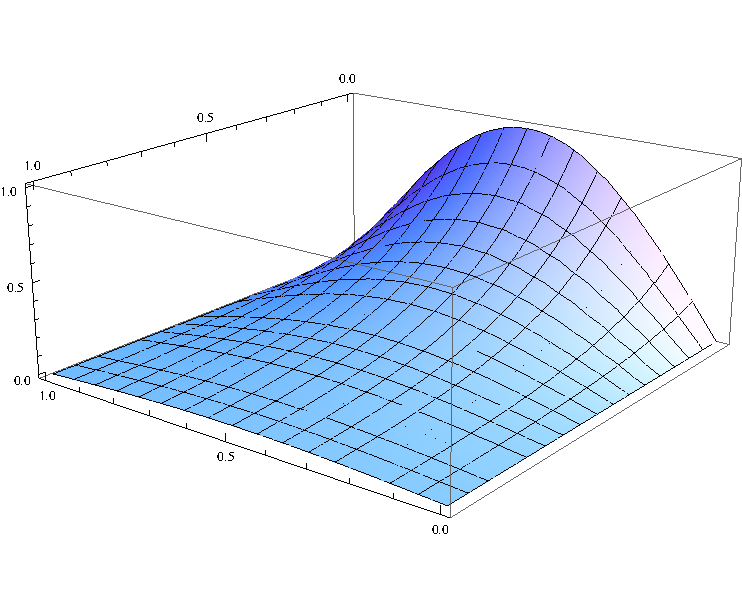
\includegraphics[width=0.9\linewidth]{figures/laplace-example.pdf}
    \label{fig:reduction-shared}
  \end{figure}
%
\end{frame}


% --------------------------------------
% parallelizing
\begin{frame}[fragile]
%
  \frametitle{Implementation strategy}
%
  \begin{itemize}
%
  \item grid resolution:
    \begin{itemize}
     \item ideally determined by analyzing the boundary conditions, since discrete sampling may
       wash out sharp features
     \item for our simple example, this can be done as part of the solver initialization
     \item we will use an $N \times N$ grid and let $N$ be user specified so we can control the
       problem size
       \begin{equation}
         \delta_{x} = \delta_{y} = \frac{1}{N-1}
       \end{equation}
     \end{itemize}
%
  \item data layout
    \begin{itemize}
    \item investigate the effect of data locality by trying out various layouts
    \end{itemize}
%
  \item setting up the update
    \begin{itemize}
      \item we only need to keep track of two iterants
      \item can be done in place; do you see how?
    \end{itemize}
%
  \item convergence criterion
    \begin{itemize}
    \item we will stop iterating when
      \begin{equation}
        \maximum{\Omega} (\phi_{t} - \phi_{t-1})) < \epsilon
      \end{equation}
      and let the user specify $\epsilon$
    \end{itemize}
%
  \end{itemize}
% 
\end{frame}

%
% \begin{figure}
%   \centering
%   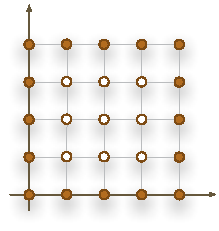
\includegraphics[scale=0.5]{figures/structured-dirichlet.pdf}
% \end{figure}

% --------------------------------------
% parallelization
\begin{frame}[fragile]
%
  \frametitle{Parallelization}
%
  \begin{itemize}
%
  \item the finest grain of work is clearly the cell update based on the value of its four
    nearest neighbors
%
  \item the shared memory implementation requires
    \begin{itemize}
    \item a scheme so that threads can update cells without the need for locks
    \item while maximizing locality of data access
    \item even the computation of the convergence criterion can be parallelized
    \end{itemize}
%
  \item with \mpi
    \begin{itemize}
    \item must partition the mesh among processes
    \item each process work on its own subgrid
    \item communication is required every iteration
    \item parallel convergence testing involves a collective operation
    \end{itemize}
%
  \end{itemize}
%
  \begin{figure}
    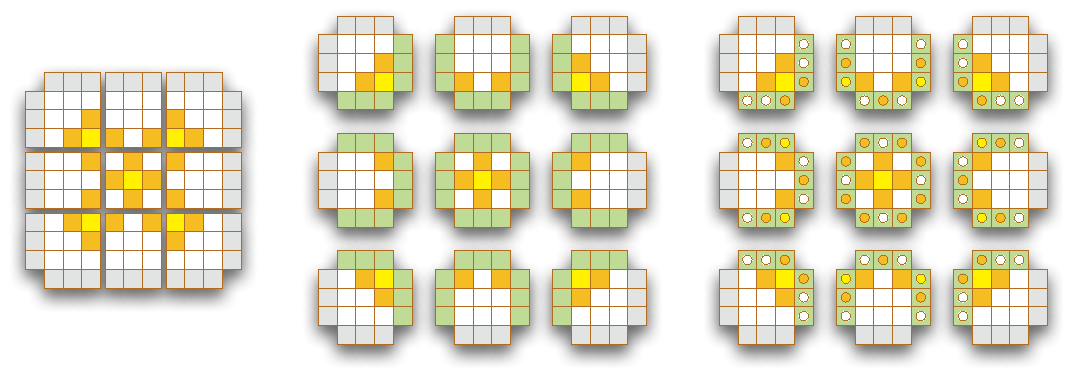
\includegraphics[scale=0.4]{figures/structured-partitioning.pdf}
  \end{figure} 
% 
\end{frame}

% --------------------------------------
% sequential
\begin{frame}[fragile]
%
  \frametitle{Sequential implementation - user interface}
%
  \begin{lstlisting}[language=c++,name=seq:frame,firstnumber=77]
// main program
int main(int argc, char* argv[]) {
    // default values for our user configurable settings
    size_t N = 10;
    double tolerance = 1.0e-6;
    const char* filename = "laplace.csv";

    // read the command line
    int command;
    while ((command = getopt(argc, argv, "N:e:o:")) != -1) {
        switch (command) {
        // get the convergence tolerance
        case 'e':
            tolerance = atof(optarg);
            break;
        // get the grid size
        case 'N':
            N = (size_t) atof(optarg);
            break;
        // get the name of the output file
        case 'o':
            filename = optarg;
        }
    }
    
  \end{lstlisting}
% 
\end{frame}

% --------------------------------------
% sequential
\begin{frame}[fragile]
%
  \frametitle{Sequential implementation - driving the solver}
%
  \begin{lstlisting}[language=c++,name=seq:frame]
    // allocate space for the solution
    Grid potential(N);

    // initialize and apply our boundary conditions
    initialize(potential);

    // call the solver
    laplace(potential, tolerance);

    // open a stream to hold the answer
    std::fstream output(filename, std::ios_base::out);

    // build a visualizer and render the solution in our chosen format
    Visualizer visualizer;
    visualizer.csv(potential, output);

    // all done
    return 0;
}
  \end{lstlisting}
% 
\end{frame}

% --------------------------------------
% sequential
\begin{frame}[fragile]
%
  \frametitle{Sequential implementation - the preamble}
%
  \begin{itemize}
  \item back up to the beginning of the file
    \begin{lstlisting}[language=c++,name=seq:frame, firstnumber=1]
#include <getopt.h>
#include <cmath>
#include <cstdlib>
#include <fstream>
#include <iostream>

// forward declarations
class Grid;
class Visualizer;

// the solver; does nothing for the time being
void initialize(Grid & grid) {};
void laplace(Grid & grid, double tolerance){};

    \end{lstlisting}
%
  \item we have separated out {\em visualization} in a different object to support different
    formats without disturbing the data representation
%
  \item \identifier{initialize} and \identifier{laplace} have trivial implementations for now
    \begin{itemize}
    \item enables testing the scaffolding without worrying about the solver
      implementation just yet
    \end{itemize}
  \end{itemize}
% 
\end{frame}

% --------------------------------------
% sequential
\begin{frame}[fragile]
%
  \frametitle{Sequential implementation - the grid object stub}
%
  \begin{lstlisting}[language=c++,name=seq:frame]
// the solution representation
class Grid {
    // interface: TBD
public:

    // meta methods
public:
    Grid(size_t size);
    ~Grid();

    // private data members: TBD
private:

    // disabled interface
    // grid will own dynamic memory, so don't let the compiler screw up
private:
    Grid(const Grid &);
    const Grid & operator= (const Grid &);
};

// the grid implementation
Grid::Grid(size_t size) {
}

Grid::~Grid() {
}

  \end{lstlisting}
% 
\end{frame}

% --------------------------------------
% sequential
\begin{frame}[fragile]
%
  \frametitle{Sequential implementation - the visualizer stub}
%
  \begin{lstlisting}[language=c++,name=seq:frame, firstnumber=97]
// the visualizer class
class Visualizer {
    // local type aliases
public:
    typedef std::ostream stream_t;

    // interface
public:
    void csv(const Grid & grid, stream_t & stream);

    // meta methods
public:
    inline Visualizer() {}
};

// the Visualizer class implementation
void Visualizer::csv(const Grid & grid, Visualizer::stream_t & stream) {
    return;
}
  \end{lstlisting}
%

\begin{itemize}
\item the code now compiles and links
  \begin{itemize}
  \item consistency check that the object collaborations are ok, for now
  \item can be tested for command line option parsing
  \end{itemize}
\end{itemize}
% 
\end{frame}

% end of file 
